\documentclass[fontsize=12pt,paper=a4,twoside]{scrartcl}

\newcommand{\grad}{\ensuremath{^{\circ}} }
\renewcommand{\strut}{\vrule width 0pt height5mm depth2mm}

\usepackage[utf8]{inputenc}
\usepackage[final]{pdfpages}
% obere Seitenränder gestalten können
\usepackage{fancyhdr}
\usepackage{moreverb}
% Graphiken als jpg, png etc. einbinden können
\usepackage{graphicx}
\usepackage{stmaryrd}
% Floats Objekte mit [H] festsetzen
\usepackage{float}
% setzt URLs schön mit \url{http://bla.laber.com/~mypage}
\usepackage{url}
% Externe PDF's einbinden können
\usepackage{pdflscape}
% Verweise innerhalb des Dokuments schick mit " ... auf Seite ... "
% automatisch versehen. Dazu \vref{labelname} benutzen
\usepackage[ngerman]{varioref}
\usepackage[ngerman]{babel}
\usepackage{ngerman}
% Bibliographie
\usepackage{bibgerm}
% Tabellen
\usepackage{tabularx}
\usepackage{supertabular}
\usepackage[colorlinks=true, pdfstartview=FitV, linkcolor=blue,
            citecolor=blue, urlcolor=blue, hyperfigures=true,
            pdftex=true]{hyperref}
\usepackage{bookmark}

\newboolean{langversion} %Deklaration
\setboolean{langversion}{true} %Zuweisung ist 'false' für Blockkurs
\newcommand{\highlight}[1]{\textcolor{blue}{\textbf{#1}}}
\newcommand{\nurlangversion}[0]{%
\ifthenelse{\boolean{langversion}}{\highlight{Muss in SWP-2 ausgefüllt werden}}{\highlight{Entfällt in SWP-1}}}

\newcommand{\swp}[0]{\ifthenelse{\boolean{langversion}}%
{Software-Projekt 2}{Software-Projekt 1}}
\newcommand{\jahr}[0]{2013}
\newcommand{\semester}[0]{\ifthenelse{\boolean{langversion}}{WiSe}{SoSe} \jahr}

% Damit Latex nicht zu lange Zeilen produziert:
\sloppy
%Uneinheitlicher unterer Seitenrand:
%\raggedbottom

% Kein Erstzeileneinzug beim Absatzanfang
% Sieht aber nur gut aus, wenn man zwischen Absätzen viel Platz einbaut
\setlength{\parindent}{0ex}

% Abstand zwischen zwei Absätzen
\setlength{\parskip}{1ex}

% Seitenränder für Korrekturen verändern
\addtolength{\evensidemargin}{-1cm}
\addtolength{\oddsidemargin}{1cm}

\bibliographystyle{gerapali}

% Lustige Header auf den Seiten
  \pagestyle{fancy}
  \setlength{\headheight}{70.55003pt}
  \fancyhead{}
  \fancyhead[LO,RE]{\swp\\ \semester{}
  \\Anforderungsspezifikation}
  \fancyhead[LE,RO]{Seite \thepage\\\slshape \leftmark\\\slshape \rightmark}

%
% Und jetzt geht das Dokument los....
%

\begin{document}

% Lustige Header nur auf dieser Seite
  \thispagestyle{fancy}
  \fancyhead[LO,RE]{ }
  \fancyhead[LE,RO]{Universität Bremen\\FB 3 -- Informatik\\
  Prof. Dr. Rainer Koschke \\TutorIn: Sabrina Wilske}
  \fancyfoot[C]{}

% Start Titelseite
  \vspace{3cm}

  \begin{minipage}[H]{\textwidth}
  \begin{center}
  \bf
  \Large
  \swp{} \jahr\\
  \smallskip
  \small
  VAK 03-BA-901.02\\
  \vspace{3cm}
  \end{center}
  \end{minipage}
  \begin{minipage}[H]{\textwidth}
  \begin{center}
  \vspace{1cm}
  \bf
  {\Large Anforderungsspezifikation}\\
  \vspace{3ex}
  \small IT\_R3V0LUT10N\\
  \vfill
  \end{center}
  \end{minipage}
  \vfill
  \begin{minipage}[H]{\textwidth}
  \begin{center}
  \sf
  \begin{tabular}{lrr}
  Sebastian Bredehöft & sbrede@tzi.de & 2751589\\
  Patrick Damrow & damsen@tzi.de & 2056170\\
  Tobias Dellert & tode@tzi.de & 2936941\\
  Tim Ellhoff & tellhoff@tzi.de & 2520913\\
  Daniel Pupat & dpupat@tzi.de & 2703053\\
  \end{tabular}
  \\ ~
  \vspace{2cm}
  \\
  \it Abgabe: 17. November 2013 --- Version 1.1\\ ~
  \end{center}
  \end{minipage}

% Ende Titelseite

% Start Leerseite

\newpage

  \thispagestyle{fancy}
  \fancyhead{}
  \fancyhead[LO,RE]{\swp{}\\ \semester{} \jahr{}
  \\Anforderungsspezifikation}
  \fancyhead[LE,RO]{Seite \thepage\\\slshape \leftmark\\~}
  \fancyfoot{}
  \renewcommand{\headrulewidth}{0.4pt}
  \tableofcontents

\newpage

  \fancyhead[LE,RO]{Seite \thepage\\\slshape \leftmark\\\slshape \rightmark}


%%%%%%%%%%%%%%%%%%%%%%%%%%%%%%%%%%%%%%%%%%%%%%%%%%%%%%%%%%%%%%%%%%%%%%%%
\section*{Version und Änderungsgeschichte}

{\em Die aktuelle Versionsnummer des Dokumentes sollte eindeutig und gut zu
identifizieren sein, hier und optimalerweise auf dem Titelblatt.}

\begin{tabular}{ccl}
Version & Datum & Änderungen \\
\hline
1.0 & TT.MM.JJJJ & Projektplan als \LaTeX Vorlage kopiert.\\
1.1 & 31.10.2013 & Charakteristika der Benutzer\\
1.2 & 01.11.2013 & System- und Hardwareschnittstellen \\
\end{tabular}


%%%%%%%%%%%%%%%%%%%%%%%%%%%%%%%%%%%%%%%%%%%%%%%%%%%%%%%%%%%%%%%%%%%%%%%%
\section{Einleitung}

Dieses Dokument spezifiziert die Anforderungen des auszuliefernden 
Produkts, welche in Zusammenarbeit mit dem Kunden der Oberschule 
Rockwinkel und den Verantwortlichen der Veranstaltung Software Projekt 2 
der Universität Bremen im Wintersemester 2013/14 erarbeitet wurden.

{\em Dieses Dokument dient als Vorlage für Eure
  Anforderungsspezifikation. Die Gliederung dieses
  Dokuments ist an die Struktur des IEEE-Standards 830.1998 angelehnt,
  weicht jedoch an einigen Stellen davon ab. Die Abweichungen sind
  im weiteren Verlauf dieses Dokuments dokumentiert. Weitere detaillierte
  Hinweise finden sich im IEEE-Standard 830.1998, der in Stud.IP      
  beziehungsweise über die Uni-Bibliothek in digitaler Form verfügbar ist
  \footnote{Bei \url{http://ieeexplore.ieee.org} im Suchfeld 'IEEE std    
   830-1998' eingeben. Funktioniert nur innerhalb des Uni-Netzes.}.}

\subsection{Zweck}
\nurlangversion

  {\em Was ist der Zweck dieser Anforderungsspezifikation? Wer sind
  die LeserInnen?}

\subsection{Rahmen}
\nurlangversion

  {\em Dieser Abschnitt soll einen groben Überblick über die zu
  erstellende Software geben: Welche Produkte sind zu erstellen (mit
  Namen)? Was tut die Software? Auch: Was tut sie nicht? Wozu soll die
  Software verwendet werden?  (Ziele etc.)}

\subsection{Definitionen, Akronyme und Abkürzungen}
\nurlangversion

  {\em Hier geht es vor allem um Begriffe aus der Anwendungsdomäne,
  d.h.\ aus der Welt des Kunden. Aber auch Begriffe, die dem Kunden
  evtl.\ fremd oder unklar sind, sollten erläutert werden.}


\subsection{Referenzen}
  {\em Neben sonstigen Quellen, die Ihr verwendet habt, können dies
  z.B.\ das Skript, dieses Beispieldokument, der zugrunde
  liegende IEEE-Standard und anderes sein}
  

\subsection{Übersicht über das Dokument}
\nurlangversion

  {\em Was enthält die Anforderungsspezifikation? Wie ist das Dokument
  organisiert?}


\section{Allgemeine Beschreibung}
\label{ch:AllgemeineBeschreibung}

\subsection{Ergebnisse der Ist-Analyse}
\nurlangversion

  {\em Hier sollten die Ergebnisse Eurer Ist-Analyse kurz
  zusammengefasst werden. Diese Beschreibung ist hilfreich, um die
  Motivation für die Anforderungen zu verstehen und um sie später
  nachzuvollziehen (z.B.\ dann wenn Anforderungen überarbeitet werden
  sollen, weil sich ihre Rahmenbedingungen geändert haben).
  
  Mögliche Inhalte: 
  \begin{itemize}
    \item Interview/Beobachtung des Kunden oder der Benutzer
    \item Analyse des bisherigen Systems und dessen Probleme 
    \item Analyse ähnlicher Systeme
    \item Auswertung der Benutzerbefragung
    \item Wie sollen die identifizierten Probleme vom neuen System adressiert werden?
  \end{itemize}
  
  N.B.: Dieser Abschnitt ist im IEEE-Standard nicht vorgesehen, aber dennoch
  sinnvoll.}

\subsubsection{Erstes Kundengespräch vom TT.MM.JJJJ}
\nurlangversion

\subsubsection{Interview mit einem Mitarbeiter der ...}
\nurlangversion

{\em Falls durchgeführt}

\subsection{Produktperspektive}
  
\subsubsection{Systemschnittstellen}

  {\em Schnittstellen zu anderen Systemen, z.B.\ Datenimport/-export,
  Konfigurationsdateien, anzubindende externe Dienste und deren Schnittstelle,
  Anbieten der eigenen Funktionalität als API o.ä.}
  
  Grundsätzlich wird ein bestehendes Computersystem (nebst typischen Ein- und Ausgabegeräten) mit einem Betriebssystem vorausgesetzt, das mit den notwendigen Schnittstellen wie z.B. dem Datenim- und -export umgehen kann.
  
  \textbf{CSV-Im-/Export:}\\
  Es gibt eine Funktion, mithilfe dieser CSV-Dateien importiert werden können. Diese kann nur vom Administrator benutzt werden. Die Bücher werden anschließend in der Datenbank der Bibliothek vorhanden sein. \\
  Es ist auch möglich, CSV Dateien zu exportieren, welche dann abgespeichert werden.

\subsubsection{Benutzerschnittstelle}

  {\em GUI-Design-Richtlinien und Interaktionsmechanismen (nicht
  Screenshots aller Dialoge --- die werden in Kapitel 3 gezeigt --- aber
  evtl.\ ein Screenshot, der einen groben Überblick und Eindruck des
  GUI-Designs gibt).}

Als Schnittstelle zwischen Benutzer und Softwaresystem dient eine Internetseite, dessen Oberfläche seiner GUI als Screenshot unten dargestellt ist. \\
Die GUI weist je nach Benutzerrechten unterschiedliche Funktionalitäten auf, da es einen Unterschied ist, ob sich ein Ausleiher ins System einloggt oder ein Administrator. \\
Der Benutzer des Systems kann somit über einen Webbrowser mithilfe der typischen Eingabegeräte wie Tastatur und Maus auf diese Funktionen zugreifen und somit mit dem System interagieren. \\
Als Ausgabegerät dient selbstredend ein handelsüblicher Monitor, der in puncto Auflösung oder Größe keine besonderen, sondern nur minimalen Anforderungen (typischerweise mindestens 640x480 Pixel) genügen muss, sowie die Möglichkeit, einen Drucker einzusetzen, um beispielsweise eine Liste auszudrucken. \\
Ausgabeinteraktionsmechanismen sind in erster Linie Text sowie wenige Grafiken. 

\subsubsection{Hardwareschnittstellen} \label{hardware}
Das Softwaresystem besitzt als Schnittstelle zur Hardware das Betriebssystem des Computers bzw. des Smartphones. \\
  Es sind keine über minimale Anforderungen in Bezug auf RAM\footnote{RAM = Random Access Memory = Hauptspeicher des Computers}, Festplattenspeicher, Prozessoren oder sonstigen Hardwarespezifika hinaus erforderlich. Somit wird die Software auch auf älteren, internetfähigen Computersystemen laufen. \\
 
\subsubsection{Softwareschnittstellen}

Unser System wird grundsätzlich plattformunabhängig laufen. Voraussetzung ist, dass das Java Runtime Environment sowie das Hibernate Framework (siehe Tabelle am Ende von Punkt \ref{Tabelle}) installiert ist. \\

   \textbf{Computer:}\\
  Unser System soll auf einem Web-Browser laufen. Dabei sollte das System auf Windows laufen, welches die verwendete Plattform des Kunden ist. Dabei ist wichtig, dass alle Betriebssysteme von Windows 2000 bis Windows 8 unterstützt werden, da der Kunde Windows 2000 verwendet. Ebenfalls sollte das System Linux und MacOS unterstützen. \\
  
  \textbf{Smartphone:}\\
  Unser System unterstützt nur Geräte, auf denen Android läuft. Dabei muss  die Version 2.3 oder höher vorliegen, da somit der größte Teil der Android Geräte verwendet werden kann.\\
Im Folgenden dient eine Tabelle der Veranschaulichung von erforderlichen Softwarekomponenten nebst Version.  \\ 

\label{Tabelle}
  \begin{tabular}{|l|l|l|l|}\hline
    \textbf{Name} & \textbf{Version} & \textbf{Hersteller} & \textbf{Quelle} \\\hline
    Java Runtime & 6 Update 37 & Oracle & \url{http://java.com} \\\hline
    Hibernate & 4.3.0.Beta1 Release& JBoss Community &  
   \url{http://www.hibernate.org/}\\\hline
    \ldots & & & \\\hline
  \end{tabular}

\subsubsection{Kommunikationsschnittstellen}
\nurlangversion

{\em Anforderungen an und Bandbreite von Kommunikationsnetzwerken, öffentliche
  oder auch private IP-Adressen?}

\subsubsection{Speicherbeschränkung}
Wie schon im Punkt \ref{hardware} beschrieben, gibt es keine Speicherbeschränkungen. Ein PC, auf dem, wie beim Kunden, Windows 2000 läuft, kann also problemlos verwendet werden. Das Softwaresystem beansprucht nicht viele Ressourcen in puncto RAM oder Festplattenspeicher.

\subsubsection{Operationen (Betriebsmodi)}
\nurlangversion

  {\em Welche Betriebsmodi gibt es? Warum? Welche Benutzerklasse darf
  was in welchem Betriebsmodus (Rechte)? Was ist der Zusammenhang
  zwischen Betriebsmodus und Sicherung/Wiederherstellung von Daten?}

\subsubsection{Möglichkeiten der lokalen Anpassung}
\nurlangversion

  {\em Was kann bei Auslieferung des Systems alles konfiguriert
  werden? Z.B. Pfade, Datenbankname, Server-IP usw. Hier ist nicht
  Internationalisierung gemeint!}


\subsection{Anwendungsfälle}
  {\em Auflistung und kurze Beschreibung aller relevanten
  Anwendungsfälle. Dies soll einen Überblick über alle Anwendungsfälle
  geben, die in 3.2 detailliert beschrieben werden.}
  
\begin{itemize}
  \item \textbf{1. Programm starten}\\
  Website wird aufgerufen/ App wird gestartet. 
  \item \textbf{2. Benutzer anmelden}\\
  Ein Benutzer meldet sich an.
  \item \textbf{3. Benutzer abmelden} \\
  Ein Benutzer meldet sich ab.
  \item \textbf{4. Start anzeigen}
  \item \textbf{4.1 Leserprofil anzeigen}
  \item \textbf{4.1.1 Vormerkung bearbeiten}
  \item \textbf{5. Publikationen anzeigen}
  \item \textbf{6. Buch hinzufügen}
  \item \textbf{7. Buch ändern}
  \item \textbf{8. Buch löschen}
  \item \textbf{9. CVS-Import}
  \item \textbf{10. CVS-Export}
  \item \textbf{11. Buch suchen}
  \item \textbf{12. Einzelnes Buch anzeigen/ Detailansicht}
  \item \textbf{13. Buch bewerten}
  \item \textbf{14. Buch ausleihen}
  \item \textbf{14.1 Buchrückgabe}
  \item \textbf{15. Buch rezensieren}
  \item \textbf{16. Buch vormerken}
  \item \textbf{17. Rezension freischalten}
  \item \textbf{18. Leserliste anzeigen}
  \item \textbf{19. Leser hinzufügen}
  \item \textbf{20. Leser ändern}
  \item \textbf{21. Leser löschen}
  \item \textbf{22. CVS-Import}
  \item \textbf{23. CVS-Export}
  \item \textbf{24. Einzelnen Leser anzeigen/ Detailansicht}
  \item \textbf{24.1 Leser sperren}
  \item \textbf{25. Leser suchen}
  \item \textbf{26. Administration öffnen}
  \item \textbf{27. Bibliothekarliste anzeigen}
  \item \textbf{28. Bibliothekar hinzufügen}
  \item \textbf{29. Bibliothekar löschen}
  \item \textbf{30. Bibliothekar ändern}
  \item \textbf{31. Statistiken anzeigen}
  \item \textbf{32. Mahnungsliste anzeigen}
  \item \textbf{33. Mahnungsliste drucken}
  \item \textbf{34. Mahnungsdetails anzeigen}
  \item \textbf{35. Startseite bearbeiten}
  \item \textbf{36. Abgabedaten und Mahngebühren bearbeiten}
 \end{itemize}


\subsection{Charakteristika der Benutzer (Daniel)}
  {\em Beschreibt hier Eure typischen Benutzer. Benutzt dazu die in
  der Vorlesung vorgestellten Personas. Zur Erinnerung: Ihr beschreibt
  konkrete Personen, die Repräsentanten der verschiedenen
  Benutzertypen sind (mit Name, evtl. Wohnort, Tätigkeit, Alter, Bild,
  \ldots). Diese sollten eine gewisse Motivation haben, bestimmte
  Anwendungsfälle durchzuführen (und dort auch eingesetzt werden!).}


\begin{table}[htbp]
\caption{Benutzer}
\label{benutzer}
\begin{tabular}{|p{2,5cm}||p{2,8cm}|p{2,8cm}|p{2,8cm}|p{2,8cm}|}
\hline 
\textbf{Name(fiktiv)} & Bert Bib & Arnold Admin & Silke Schüler & Bart Besucher\\ \hline
\textbf{Bild(fiktiv)} & & & & \\ \hline
\textbf{Rolle} & Bibliothekar & Administrator & Leiherin & uregistrierter Leiher \\ \hline
\textbf{Beruf} & Bibliothekar & Bibliothekar & Schülerin & Anwalt\\ \hline
\textbf{Alter} & 39 & 56 & 16 & 34\\ \hline
\textbf{Ziel} & Bibliothek verwalten & System verwalten & Bücher ausleihen & Bücher ausleihen \\ \hline
\textbf{Verwendung der Software} & Bücher und Nutzer verwalten & System und Bibliothekare verwalten & Bücher suchen, ausleihen etc. & keine\\ \hline
\end{tabular}
\end{table}

\subsection{Einschränkungen}
\label{sec:Einschraenkungen}
  {\em Dinge, die die Entwurfsfreiheit einschränken, z.B.
  \begin{itemize}
   \item feste Vorgaben (z.B. Policies)
   \item gesetzliche Rahmenbedingungen
   \item Hardwarebeschränkungen
   \item festgelegte Schnittstellen zu anderen Anwendungen
   \item parallele Operationen (z.B. Multithreading)
   \item Prüfungs- und Steuerungsfunktionen
   \item Verlässlichkeitsanforderungen
   \item Kritikalität der Anwendung
   \item Sicherheit
  \end{itemize}
  }

\subsubsection{Rahmenbedingungen}
\nurlangversion

\subsubsection{Gesetzliche Rahmenbedingungen}
\nurlangversion
 
\subsubsection{Sicherheitskritische Aspekte}
\nurlangversion

\subsection{Annahmen und Abhängigkeiten}
\nurlangversion

  {\em Faktoren, deren Änderung zwangsläufig zu Änderungen an der
  Anforderungsspezifikation führen würde.}



\subsection{Ausblick}
\nurlangversion

  {\em Beschreibt hier knapp, welche Änderungen und Erweiterungen
  zukünftig (d.h.\ nach Auslieferung des Systems) zu erwarten sind.
  Diese Information ist wichtig für den Entwurf, um mögliche
  Änderungen frühzeitig im ersten Entwurf berücksichtigen zu können.
  Der Entwurf kann dann so gestaltet werden, dass die zukünftigen
  Anforderungen leicht realisierbar sind. Die zukünftigen
  Anforderungen sollten realistisch sein, ansonsten könnte ein unnötig
  allgemeiner und damit zu komplizierter Entwurf die Folge sein.  Auch
  dieser Abschnitt ist im IEEE-Standard nicht vorgesehen -- zumindest
  nicht explizit in Form eines eigenständigen Abschnitts. Dennoch
  handelt es sich um wertvolle Information, von der der Entwurf
  profitieren kann.}
  

\section{Detaillierte Beschreibung}
\label{ch:DetaillierteBeschreibung}
{\em Die externen Schnittstellen werden grob in Abschnitt 2
  beschrieben.  Wenn die grobe Beschreibung dort nicht genügt, kann
  sie hier detaillierter ausgeführt werden (wie vom IEEE-Standard
  vorgesehen).}

\subsection{Datenmodell}
  {\em Das Datenmodell im Kontext des Pflichtenhefts ist {\glqq}die
  Darstellung von Informationen und deren Beziehungen in einem
  fachlogischen Konzept{\grqq}. Es soll hier gezeigt werden, welche
  Einheiten für das existierende System relevant sind und welche
  Beziehungen zwischen diesen Einheiten gelten. Es handelt sich
  hierbei noch nicht um ein Datenbankschema oder eine Spezifikation
  von Klassen für die Implementierung (Entwurf), sondern um die
  Modellierung der realen Welt. Das Datenmodell ist leitend für den
  Entwurf (weil alles darin beschrieben sich auch in der Software 
  wiederfinden wird), aber nimmt den Entwurf nicht schon vorweg.
  
  Das Datenmodell soll als UML-Klassendiagramm angegeben werden.
  Wichtig ist hierbei die korrekte Verwendung der UML: Klassen,
  Attribute, Generalisierung, Assoziation, Aggregation, Komposition,
  Multiplizitäten. Außerdem sollte das Diagramm sinnvoll und gut
  lesbar sein. Dazu gehört weiterhin eine kurze Beschreibung des
  Modells mit ergänzenden Informationen, insbesondere wenn die
  Relationen durch ihren Namen nicht selbsterklärend sind. Gebt
  unbedingt ein Mengengerüst für die Daten an: Wie viele Instanzen der
  wichtigsten Klassen werden erwartet? Erwartet Ihr Änderungen im
  Datenvolumen in der Zukunft?}


\subsection{Anwendungsfälle}
\begin{figure}[htbp]
\caption{Startseite}
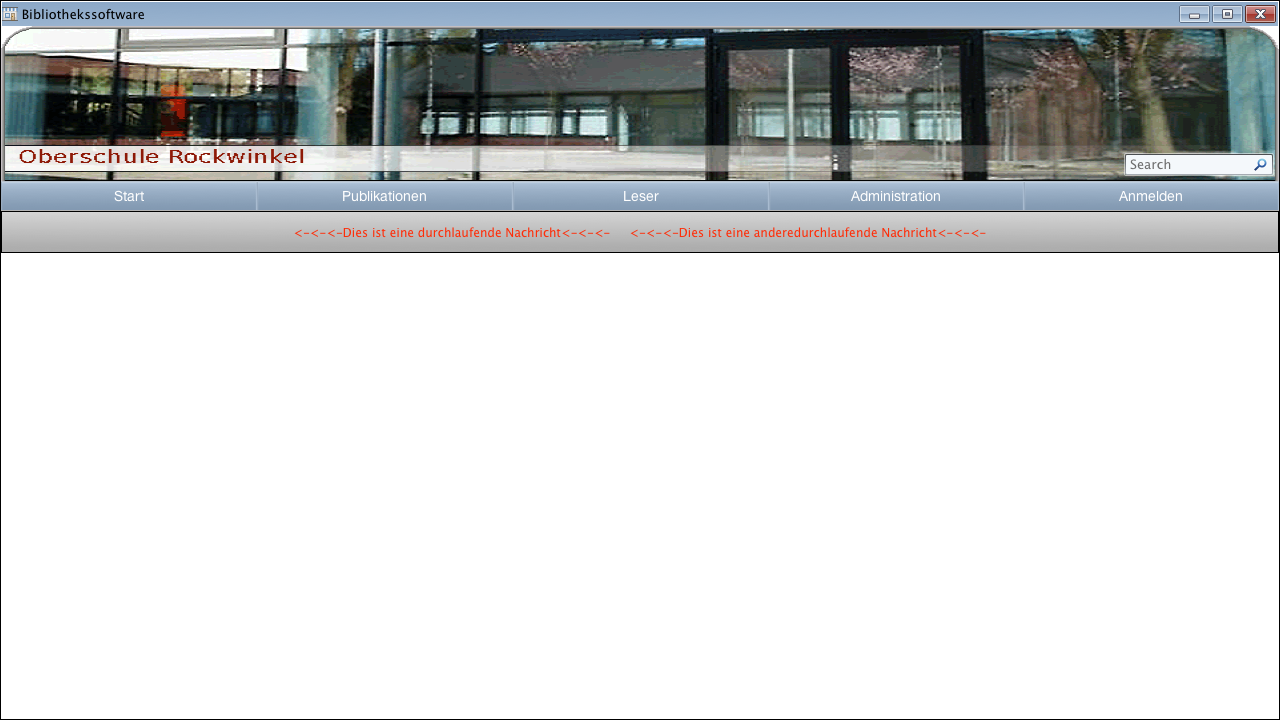
\includegraphics[width=1\textwidth]{WebApp-Screens/Startscreen-loggedOut.png}
  \label{startseite}
\end{figure}

\begin{table}[htbp]
\label{1}
\begin{tabular}{|l|p{10cm}|}
\hline 
\textbf{1} & \textbf{Programm starten} \\ \hline
\textbf{Akteure} & Bert Bib, Arnold Admin, Silke Schüler, Bart Besucher\\ \hline
\textbf{Ziel} & Der Akteur möchte das Programm starten  \\ \hline
\textbf{Vorbedingungen} & keine \\ \hline
\textbf{Regulärer Ablauf} & 
1. Der Akteur startet das Programm, indem er die URL aufruft \\
&2. Das Programm startet und zeigt die Startseite \\ \hline
\textbf{Varianten} & keine \\ \hline
\textbf{Nachbedingungen} & Das Programm ist gestartet und der Benutzer kann dieses nun verwenden \\ \hline
\textbf{Fehler-/Ausnahmefälle} & Server ist nicht erreichbar \\ \hline
\end{tabular}
\end{table}

\begin{figure}[htbp]
\caption{Loginscreen}
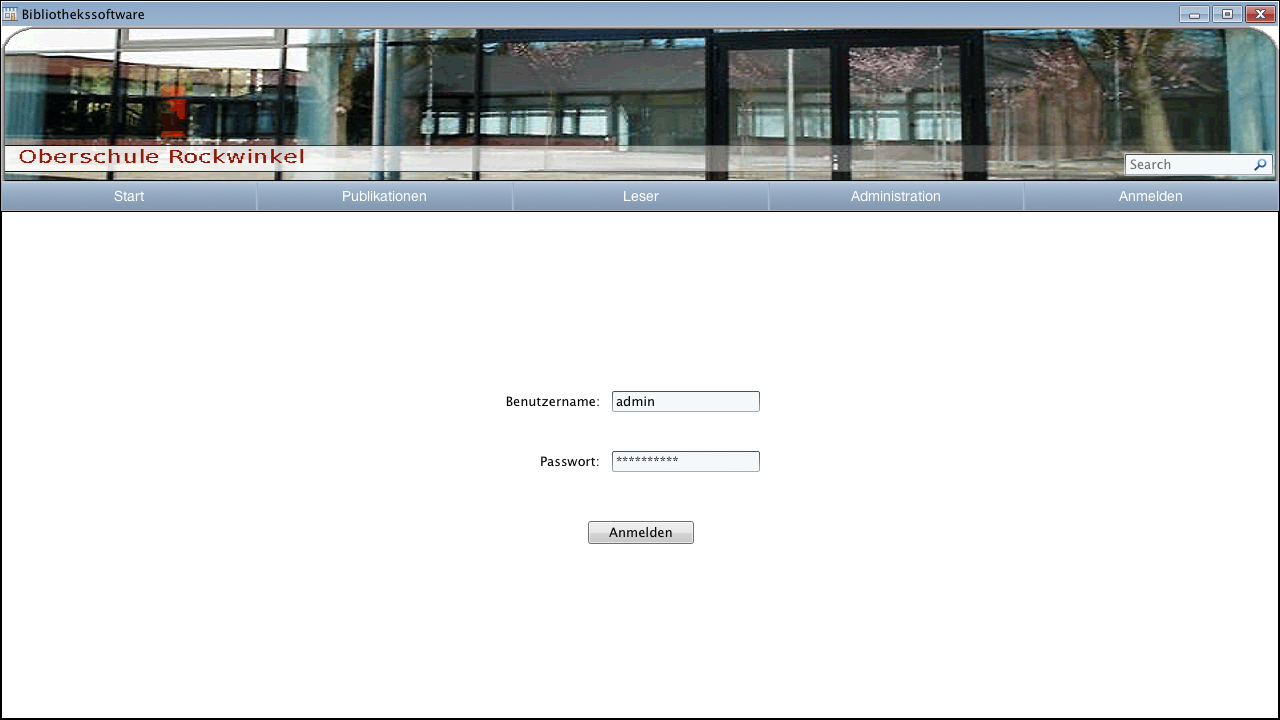
\includegraphics[width=1\textwidth]{WebApp-Screens/Loginscreen.png}
  \label{login}
\end{figure}

\begin{table}[htbp]
\label{2}
\begin{tabular}{|l|p{10cm}|}
\hline 
\textbf{2} & \textbf{Benutzer anmelden} \\ \hline
\textbf{Akteure} & Bert Bib, Arnold Admin, Silke Schüler, Bart Besucher\\ \hline
\textbf{Ziel} & Der Akteur möchte sich im System anmelden  \\ \hline
\textbf{Vorbedingungen} & Das Programm wurde gestartet  \\ \hline
\textbf{Regulärer Ablauf} & 
1. Bib gibt seinen Benutzernamen und sein Passwort ein \\
&2. Bert Bib drückt auf den Button anmelden\\
&3. Der Startbildschirm erscheint wieder und Bert Bib kann nun alle Funktionen eines Bibliothekars verwenden\\ \hline
\textbf{Varianten} & 
1. Arnold Admin gibt seinen Benutzernamen und sein Passwort ein \\
&2. Arnold Admin drückt auf den Button 'Anmelden'\\
&3. Der Startbildschirm erscheint wieder und Arnold Admin kann nun alle Funktionen eines Administrators verwenden\\  
& \\
&1. Silke Schüler gibt ihren Benutzernamen und ihr Passwort ein \\
&2. Silke Schüler drückt auf den Button 'Anmelden'\\
&3. Der Startbildschirm erscheint wieder und Silke Schüler kann nun alle Funktionen eines registrierten Nutzers verwenden\\ \hline
\textbf{Nachbedingungen} & Die Personen sind nun angemeldet und können nun Funktionen abhängig vom Zugriffsrecht verwenden \\ \hline
\textbf{Fehler-/Ausnahmefälle} & 
1. Bart Besucher besitzt kein Benutzernamen oder Passwort, somit kann er sich nicht anmelden und hat keinen Zugriff auf die anderen Funktionen \\
&2. Es wird der falsche Nutzername oder das falsche Passwort eingegeben. Dann erscheint eine Fehlermeldung, welche dieses Problem beschreibt \\ \hline
\end{tabular}
\end{table}

\begin{table}[htbp]
\label{3}
\begin{tabular}{|l|p{10cm}|}
\hline 
\textbf{3} & \textbf{Benutzer abmelden} \\ \hline
\textbf{Akteure} & Bert Bib, Arnold Admin, Silke Schüler \\ \hline
\textbf{Ziel} & Der Akteur möchte sich vom System abmelden  \\ \hline
\textbf{Vorbedingungen} & Der Benutzer ist angemeldet  \\ \hline
\textbf{Regulärer Ablauf} & 
1. Ein Benutzer drückt auf den Button 'Abmelden' \\
&2. Das System meldet den Benutzer ab\\
\hline
\textbf{Varianten} & 
keine \\ \hline
\textbf{Nachbedingungen} & Es wird nun die Startseite angezeigt und der Benutzer ist abgemeldet \\ \hline
\textbf{Fehler-/Ausnahmefälle} & keine
\end{tabular}
\end{table}

\begin{figure}[htbp]
\caption{Startseite bei angemeldeten Benutzer}
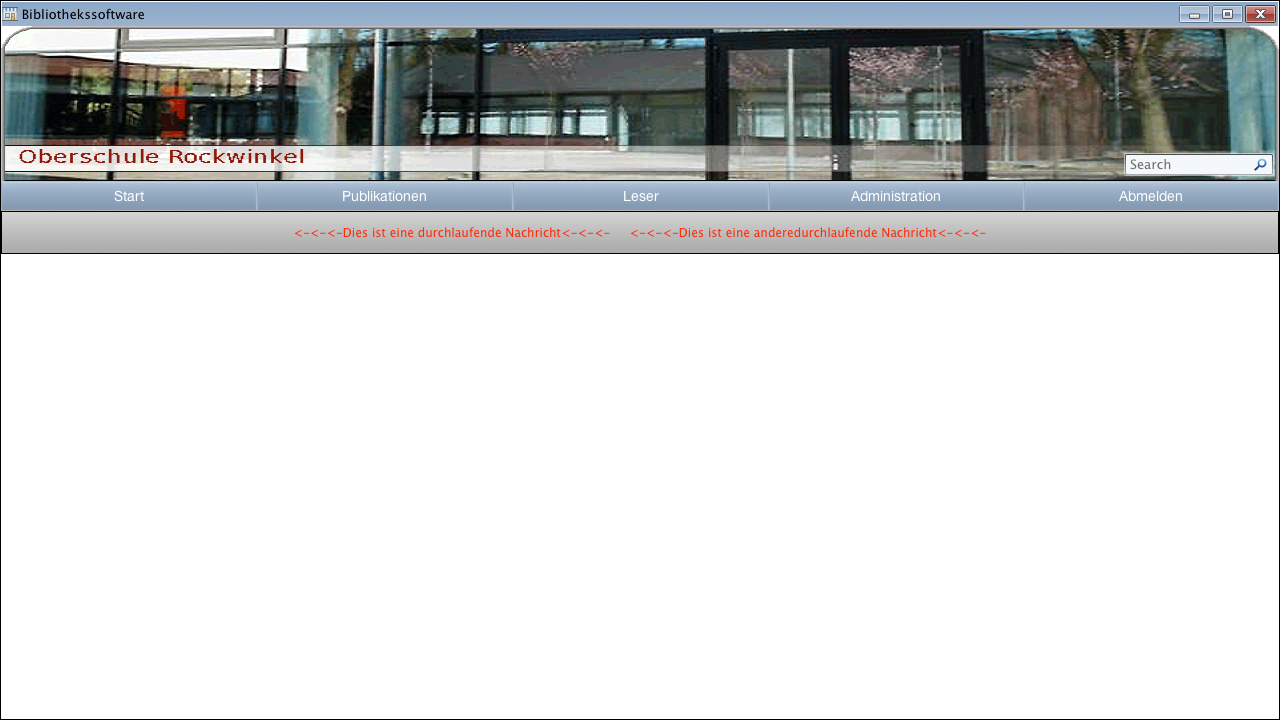
\includegraphics[width=1\textwidth]{WebApp-Screens/Startscreen-loggedIn.png}
  \label{startlog}
\end{figure}

\begin{table}[htbp]
\label{4}
\begin{tabular}{|l|p{10cm}|}
\hline 
\textbf{4} & \textbf{Startseite anzeigen} \\ \hline
\textbf{Akteure} & Bert Bib, Arnold Admin, Silke Schüler, Bart Besucher\\ \hline
\textbf{Ziel} & Der Akteur möchte die Startseite des Systems aufrufen  \\ \hline
\textbf{Vorbedingungen} & Das Programm wurde gestartet  \\ \hline
\textbf{Regulärer Ablauf} & 
1. Ein Benutzer drückt auf den Button 'Start' \\
&2. Das System zeigt die Startseite an\\
\hline
\textbf{Varianten} & 
Anwendungsfall 1 \\ \hline
\textbf{Nachbedingungen} & Es wird nun die Startseite angezeigt \\ \hline
\textbf{Fehler-/Ausnahmefälle} & keine\\
\hline
\end{tabular}
\end{table}

\begin{figure}[htbp]
\caption{Publikationsscreen von Silke Schüler oder Bart Besucher}
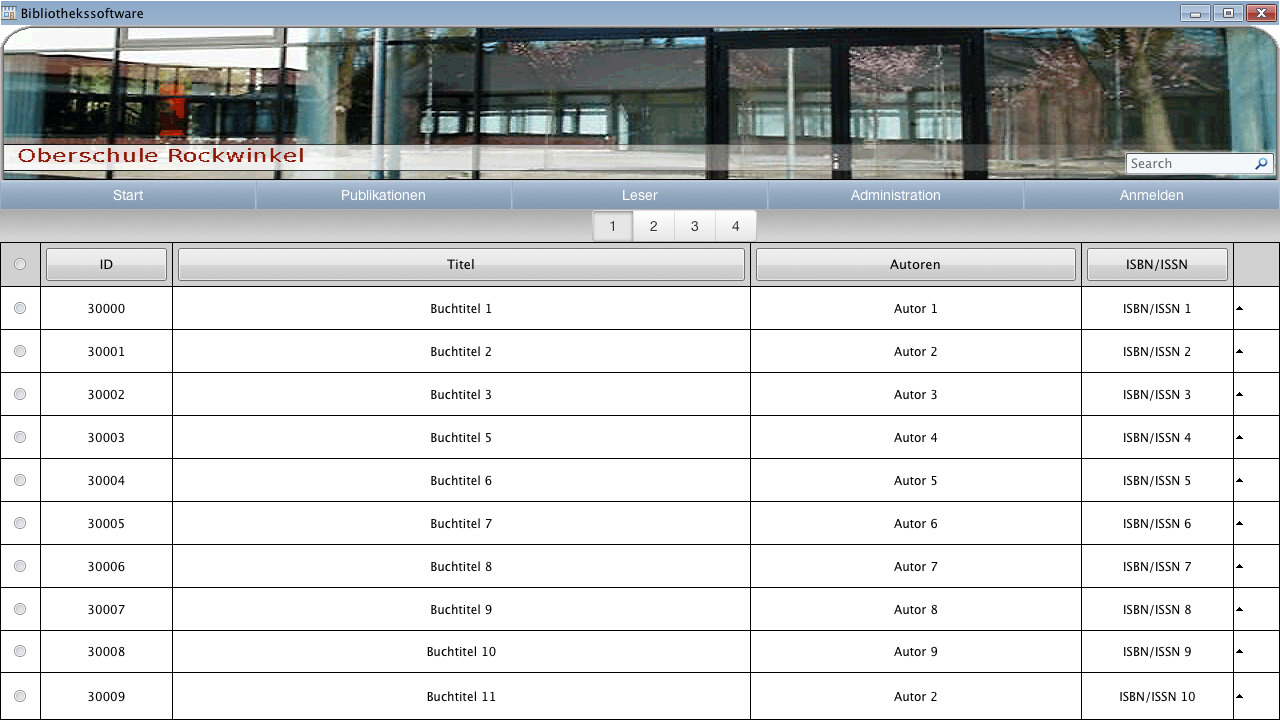
\includegraphics[width=1\textwidth]{WebApp-Screens/PublicationsscreenLogOut.png}
  \label{pub}
\end{figure}

\begin{table}[htbp]
\label{4.1}
\begin{tabular}{|l|p{10cm}|}
\hline 
\textbf{4.1} & \textbf{Leserprofil anzeigen} \\ \hline
\textbf{Akteure} & Silke Schüler\\ \hline
\textbf{Ziel} & Der Akteur möchte sich das eigene Leserprofil anzeigen lassen  \\ \hline
\textbf{Vorbedingungen} & Der Akteur ist angemeldet  \\ \hline
\textbf{Regulärer Ablauf} & 
1. Ein Benutzer drückt auf den Button 'Profil' \\
&2. Das System zeigt die Profilseite an\\
\hline
\textbf{Varianten} & 
keine \\ \hline
\textbf{Nachbedingungen} & Es wird nun die Profilseite angezeigt \\ \hline
\textbf{Fehler-/Ausnahmefälle} & keine\\
\hline
\end{tabular}
\end{table}

\begin{table}[htbp]
\label{4.1.1}
\begin{tabular}{|l|p{10cm}|}
\hline 
\textbf{4.1.1} & \textbf{Vormerkung bearbeiten} \\ \hline
\textbf{Akteure} & Silke Schüler\\ \hline
\textbf{Ziel} & Der Akteur möchte die eigenen Vormerkungen bearbeiten  \\ \hline
\textbf{Vorbedingungen} & Der Benutzer hat sein Profil geöffnet  \\ \hline
\textbf{Regulärer Ablauf} & 
1. Ein Benutzer drückt auf den Button 'Vormerkungen' \\
&2. Das System zeigt eine Liste der Vormerkungen an\\
\hline
\textbf{Varianten} & 
keine \\ \hline
\textbf{Nachbedingungen} & Es wird nun die Vormerkungen angezeigt, die bearbeitet werden können \\ \hline
\textbf{Fehler-/Ausnahmefälle} & keine\\
\hline
\end{tabular}
\end{table}

\begin{table}[htbp]
\label{5}
\begin{tabular}{|l|p{10cm}|}
\hline 
\textbf{5} & \textbf{Publikationen anzeigen} \\ \hline
\textbf{Akteure} & Bert Bib, Arnold Admin, Silke Schüler, Bart Besucher\\ \hline
\textbf{Ziel} & Der Akteur möchte die Liste der Publikationen aufrufen  \\ \hline
\textbf{Vorbedingungen} & Das Programm wurde gestartet  \\ \hline
\textbf{Regulärer Ablauf} & 
1. Ein Benutzer drückt auf den Button 'Publikationen' \\
&2. Das System zeigt die Publikationsliste an\\
\hline
\textbf{Varianten} & 
keine \\ \hline
\textbf{Nachbedingungen} & Es wird nun die Liste mit den Publikationen angezeigt \\ \hline
\textbf{Fehler-/Ausnahmefälle} & keine\\
\hline
\end{tabular}
\end{table}

\begin{table}[htbp]
\label{6}
\begin{tabular}{|l|p{10cm}|}
\hline 
\textbf{6} & \textbf{Buch hinzufügen} \\ \hline
\textbf{Akteure} & Bert Bib\\ \hline
\textbf{Ziel} & Der Akteur möchte ein neues Buch hinzufügen \\ \hline
\textbf{Vorbedingungen} & Der Akteur ist als Bibliothekar angemeldet und hat die Publikationsliste aufgerufen  \\ \hline
\textbf{Regulärer Ablauf} & 
1. Der Benutzer drückt auf den Button 'Hinzufügen' \\
&2. Das System zeigt das Formular für das Hinzufügen eines Buches an\\
&3. Der Benutzer drückt den Button 'Speichern'\\
\hline
\textbf{Varianten} & 
keine \\ \hline
\textbf{Nachbedingungen} & Das Buch wurde gespeichert und ist in die Datenbank aufgenommen worden\\ \hline
\textbf{Fehler-/Ausnahmefälle} & 1. falsches ISBN-Format wurde eingeben\\
&2. Pflichtfelder wurden nicht eingegeben\\
\hline
\end{tabular}
\end{table}

\begin{table}[htbp]
\label{7}
\begin{tabular}{|l|p{10cm}|}
\hline 
\textbf{7} & \textbf{Buch ändern} \\ \hline
\textbf{Akteure} & Bert Bib\\ \hline
\textbf{Ziel} & Der Akteur möchte ein Daten eines Buches ändern \\ \hline
\textbf{Vorbedingungen} & Der Akteur ist als Bibliothekar angemeldet und hat die Detailsicht eines Buches aufgerufen  \\ \hline
\textbf{Regulärer Ablauf} & 
1. Der Benutzer drückt auf den Button 'Ändern' \\
&2. Das System zeigt das Formular für das Hinzufügen eines Buches an\\
&3. Der Benutzer drückt den Button 'Änderung speichern'\\
\hline
\textbf{Varianten} & 
keine \\ \hline
\textbf{Nachbedingungen} & Die Änderungen wurden gespeichert und sind in die Datenbank aufgenommen worden\\ \hline
\textbf{Fehler-/Ausnahmefälle} & 1. falsches ISBN-Format wurde eingeben\\
&2. Pflichtfelder wurden nicht eingegeben\\
\hline
\end{tabular}
\end{table}

\begin{table}[htbp]
\label{8}
\begin{tabular}{|l|p{10cm}|}
\hline 
\textbf{8} & \textbf{Buch löschen} \\ \hline
\textbf{Akteure} & Bert Bib\\ \hline
\textbf{Ziel} & Der Akteur möchte ein Buch löschen \\ \hline
\textbf{Vorbedingungen} & Der Akteur ist als Bibliothekar angemeldet und hat die Publikationsliste aufgerufen  \\ \hline
\textbf{Regulärer Ablauf} & 
1. Der Benutzer markiert die zu löschenden Bücher\\
&2. Der Benutzer drückt auf den Button 'Löschen' \\
\hline
\textbf{Varianten} & 
1. Der Benutzer befindet sich in der Detailsicht eines Buches\\
&2. Der Benutzer drückt auf den Button 'Löschen' \\ \hline
\textbf{Nachbedingungen} & Das Buch wurde gelöscht \\ \hline
\textbf{Fehler-/Ausnahmefälle} & \\
\hline
\end{tabular}
\end{table}

\begin{table}[htbp]
\label{9}
\begin{tabular}{|l|p{10cm}|}
\hline 
\textbf{9} & \textbf{CVS-Import} \\ \hline
\textbf{Akteure} & Bert Bib\\ \hline
\textbf{Ziel} & Der Akteur möchte eine CVS-Datei für Bücher importieren \\ \hline
\textbf{Vorbedingungen} & Der Akteur ist als Bibliothekar angemeldet und hat die Publikationsliste aufgerufen \\ \hline
\textbf{Regulärer Ablauf} & 
1. Der Benutzer drückt auf den Button CVS-Import \\
&2. Der Benutzer kann nun eine CVS-Datei auswählen\\
&3. Der Benutzer drückt den Button 'Importieren'\\
\hline
\textbf{Varianten} & 
keine \\ \hline
\textbf{Nachbedingungen} & Die CVS-Datei wurde hochgeladen und in der Datenbank ergänzt\\ \hline
\textbf{Fehler-/Ausnahmefälle} & 1. falsches Datei-Format\\
\hline
\end{tabular}
\end{table}

\begin{table}[htbp]
\label{10}
\begin{tabular}{|l|p{10cm}|}
\hline 
\textbf{10} & \textbf{CVS-Export} \\ \hline
\textbf{Akteure} & Bert Bib\\ \hline
\textbf{Ziel} & Der Akteur möchte eine CVS-Datei von der Datenbank exportieren \\ \hline
\textbf{Vorbedingungen} & Der Akteur ist als Bibliothekar angemeldet und hat die Publikationsliste aufgerufen \\ \hline
\textbf{Regulärer Ablauf} & 
1. Der Benutzer drückt auf den Button CVS-Export \\
&2. Der Benutzer kann nun den Speicherort und Name für eine CVS-Datei auswählen\\
&3. Der Benutzer drückt den Button 'Exportieren'\\
\hline
\textbf{Varianten} & 
keine \\ \hline
\textbf{Nachbedingungen} & Die CVS-Datei wurde exportiert und gespeichert\\ \hline
\textbf{Fehler-/Ausnahmefälle} & keine\\
\hline
\end{tabular}
\end{table}

\begin{table}[htbp]
\label{11}
\begin{tabular}{|l|p{10cm}|}
\hline 
\textbf{11} & \textbf{Buch suchen} \\ \hline
\textbf{Akteure} & Bert Bib, Silke Schüler, Bart Besucher, Arnold Admin\\ \hline
\textbf{Ziel} & Der Akteur möchte ein Buch suchen \\ \hline
\textbf{Vorbedingungen} & keine \\ \hline
\textbf{Regulärer Ablauf} & 
1. Der Benutzer gibt den Suchbegriff in das Suchfeld ein und drückt 'Eingabe' \\
&2. Eine Liste von Büchern mit passendem Suchbegriff wird angezeigt\\
\hline
\textbf{Varianten} & 
keine \\ \hline
\textbf{Nachbedingungen} & Eine Liste von Büchern mit passendem Suchbegriff wird angezeigt\\ \hline
\textbf{Fehler-/Ausnahmefälle} & Zum eingegeben Suchbegriff existieren keine Daten\\
\hline
\end{tabular}
\end{table}

\begin{table}[htbp]
\label{12}
\begin{tabular}{|l|p{10cm}|}
\hline 
\textbf{12} & \textbf{Einzelnes Buch anzeigen/ Detailansicht} \\ \hline
\textbf{Akteure} & Bert Bib, Silke Schüler, Bart Besucher, Arnold Admin\\ \hline
\textbf{Ziel} & Der Akteur möchte sich Details zu einem Buch anzeigen lassen \\ \hline
\textbf{Vorbedingungen} & Die Publikationsliste oder die Suchliste wurde aufgerufen \\ \hline
\textbf{Regulärer Ablauf} & 
1. Der Benutzer klickt auf den Button 'Details' bei einem Buch in der Liste \\
&2. Die Detailseite des Buches wird angezeigt\\
\hline
\textbf{Varianten} & 
keine \\ \hline
\textbf{Nachbedingungen} & Die Detailseite eines Buches wird angezeigt\\ \hline
\textbf{Fehler-/Ausnahmefälle} & keine\\
\hline
\end{tabular}
\end{table}

\newpage

\begin{table}[htbp]
\label{13}
\begin{tabular}{|l|p{10cm}|}
\hline 
\textbf{13} & \textbf{Buch bewerten} \\ \hline
\textbf{Akteure} & Silke Schüler\\ \hline
\textbf{Ziel} & Der Akteur möchte ein Buch bewerten \\ \hline
\textbf{Vorbedingungen} & Die Detailansicht eines Buches wurde aufgerufen \\ \hline
\textbf{Regulärer Ablauf} & 
1. Der Benutzer klickt auf den Button 'Bewerten' und kann nun in einem Dropdownmenü eine Punktzahl auswählen\\
&2. Der Benutzer drückt den Button 'Buch bewerten'\\
\hline
\textbf{Varianten} & 
keine \\ \hline
\textbf{Nachbedingungen} & Das Buch wurde vom Akteur bewertet und lässt sich kein zweites Mal bewerten\\ \hline
\textbf{Fehler-/Ausnahmefälle} & Das Buch wurde schon einmal bewertet\\
\hline
\end{tabular}
\end{table}

\begin{table}[htbp]
\label{14}
\begin{tabular}{|l|p{10cm}|}
\hline 
\textbf{14} & \textbf{Buch ausleihen} \\ \hline
\textbf{Akteure} & Bert Bib, Silke Schüler\\ \hline
\textbf{Ziel} & Silke Schüler möchte ein Buch ausleihen \\ \hline
\textbf{Vorbedingungen} & Bert Bib ist im System als Bibliothekar angemeldet und Silke Schüler ist vor Ort \\ \hline
\textbf{Regulärer Ablauf} & 
1. Silke Schüler gibt Buch (Bücher) und ihren Bibliotheksausweis zum Einscannen an Bert Bib\\
&2. Bert Bib scannt erst den Ausweis\\
&3. Nun scannt Bert Bib die Bücher ein\\
&4. Die Liste der auszuleihenden Bücher wird mit dem Ausleiher angezeigt\\
&5. Bert Bib drückt auf den Button 'Ausleihen'\\
\hline
\textbf{Varianten} & 
keine \\ \hline
\textbf{Nachbedingungen} & Die Bücher stehen im System als 'ausgeliehen an Silke Schüler'\\ \hline
\textbf{Fehler-/Ausnahmefälle} & Silke Schüler ist gesperrt und kann keine Bücher ausleihen\\
\hline
\end{tabular}
\end{table}

\begin{table}[htbp]
\label{14.1}
\begin{tabular}{|l|p{10cm}|}
\hline 
\textbf{14.1} & \textbf{Buchrückgabe} \\ \hline
\textbf{Akteure} & Bert Bib, Silke Schüler\\ \hline
\textbf{Ziel} & Der Akteur will Bücher zurückgeben \\ \hline
\textbf{Vorbedingungen} & Bücher sind ausgeliehen \\ \hline
\textbf{Regulärer Ablauf} & 
1. Ein Akteur gibt abzugebene Bücher dem Bibliothekaren \\
&2. Der Bibliothekar scannt die Bücher ein\\
&3. Der Bibliothekar drückt auf den Button 'Bücher zurückgeben'\\
\hline
\textbf{Varianten} & 
Mahngebühren werden bezahlt \\ \hline
\textbf{Nachbedingungen} & Die Bücher stehen im System als zurückgegeben\\ \hline
\textbf{Fehler-/Ausnahmefälle} & keine\\
\hline
\end{tabular}
\end{table}

\begin{table}[htbp]
\label{14.1}
\begin{tabular}{|l|p{10cm}|}
\hline 
\textbf{14.1} & \textbf{Buchrückgabe} \\ \hline
\textbf{Akteure} & Bert Bib, Silke Schüler\\ \hline
\textbf{Ziel} & Der Akteur will Bücher zurückgeben \\ \hline
\textbf{Vorbedingungen} & Bücher sind ausgeliehen \\ \hline
\textbf{Regulärer Ablauf} & 
1. Ein Akteur gibt abzugebene Bücher dem Bibliothekaren \\
&2. Der Bibliothekar scannt die Bücher ein\\
&3. Der Bibliothekar drückt auf den Button 'Bücher zurückgeben'\\
\hline
\textbf{Varianten} & 
Mahngebühren werden bezahlt \\ \hline
\textbf{Nachbedingungen} & Die Bücher stehen im System als zurückgegeben\\ \hline
\textbf{Fehler-/Ausnahmefälle} & keine\\
\hline
\end{tabular}
\end{table}

\begin{table}[htbp]
\label{15}
\begin{tabular}{|l|p{10cm}|}
\hline 
\textbf{15} & \textbf{Buch rezensieren} \\ \hline
\textbf{Akteure} & Silke Schüler\\ \hline
\textbf{Ziel} & Der Akteur will ein Buch rezensieren \\ \hline
\textbf{Vorbedingungen} & Der Akteur befindet sich auf der Detailsicht eines Buches \\ \hline
\textbf{Regulärer Ablauf} & 
1. Der Akteur drückt auf 'Buch rezensieren' \\
&2. Der Akteur schreibt seine Rezension in das entsprechende Feld\\
&3. Der Button 'Rezension abschicken' wird gedrückt\\
\hline
\textbf{Varianten} & 
keine \\ \hline
\textbf{Nachbedingungen} & Die Rezension wird abgeschickt und der Bibliothekar muss diese nun freischalten\\ \hline
\textbf{Fehler-/Ausnahmefälle} & Es wurde nichts in das Bedienfeld eingegeben und dann abgeschickt.\\
\hline
\end{tabular}
\end{table}

\begin{table}[htbp]
\label{16}
\begin{tabular}{|l|p{10cm}|}
\hline 
\textbf{16} & \textbf{Buch vormerken} \\ \hline
\textbf{Akteure} & Silke Schüler\\ \hline
\textbf{Ziel} & Der Akteur will ein Buch vormerken \\ \hline
\textbf{Vorbedingungen} & Der Akteur befindet sich auf der Detailsicht eines Buches \\ \hline
\textbf{Regulärer Ablauf} & 
1. Der Akteur drückt auf 'Buch vormerken' \\
&2. Das Buch wurde vorgemerkt\\
\hline
\textbf{Varianten} & 
keine \\ \hline
\textbf{Nachbedingungen} & Das Buch wurde vorgemerkt und erscheint nun auf der Profilseite\\ \hline
\textbf{Fehler-/Ausnahmefälle} & Das Buch wurde bereits vorgemerkt und kann somit nicht noch einmal vorgemerkt werden\\
\hline
\end{tabular}
\end{table}

\begin{table}[htbp]
\label{17}
\begin{tabular}{|l|p{10cm}|}
\hline 
\textbf{17} & \textbf{Rezension freischalten} \\ \hline
\textbf{Akteure} & Bert Bib\\ \hline
\textbf{Ziel} & Der Bibliothekar will eine Rezension überprüfen und gegebenenfalls freischalten \\ \hline
\textbf{Vorbedingungen} & Es wurde eine Rezension geschrieben und der Bibliothekar hat diese zur Überprüfung erhalten. \\ \hline
\textbf{Regulärer Ablauf} & 
1. Der Akteur liest sich die Rezension durch \\
&2. Der Bibliothekar schaltet die Rezension frei\\
\hline
\textbf{Varianten} & 
1. Der Akteur ließt sich die Rezension durch \\
&2. Der Bibliothekar lehnt die Rezension ab \\ \hline
\textbf{Nachbedingungen} & Die Rezension wurde angenommen und freigeschaltet oder abgelehnt\\ \hline
\textbf{Fehler-/Ausnahmefälle} & \\
\hline
\end{tabular}
\end{table}

\begin{table}[htbp]
\label{18}
\begin{tabular}{|l|p{10cm}|}
\hline 
\textbf{18} & \textbf{Leserliste anzeigen} \\ \hline
\textbf{Akteure} & Bert Bib\\ \hline
\textbf{Ziel} & Der Akteur möchte die Liste der Leser aufrufen  \\ \hline
\textbf{Vorbedingungen} & Das Programm wurde gestartet  \\ \hline
\textbf{Regulärer Ablauf} & 
1. Ein Benutzer drückt auf den Button 'Leserliste' \\
&2. Das System zeigt die Leserliste an\\
\hline
\textbf{Varianten} & 
keine \\ \hline
\textbf{Nachbedingungen} & Es wird nun die Liste mit den Lesern angezeigt \\ \hline
\textbf{Fehler-/Ausnahmefälle} & keine\\
\hline
\end{tabular}
\end{table}

\begin{table}[htbp]
\label{19}
\begin{tabular}{|l|p{10cm}|}
\hline 
\textbf{19} & \textbf{Leser hinzufügen} \\ \hline
\textbf{Akteure} & Bert Bib\\ \hline
\textbf{Ziel} & Der Akteur möchte ein neuen Leser hinzufügen \\ \hline
\textbf{Vorbedingungen} & Der Akteur ist als Bibliothekar angemeldet und hat die Leserliste aufgerufen  \\ \hline
\textbf{Regulärer Ablauf} & 
1. Der Benutzer drückt auf den Button 'Hinzufügen' \\
&2. Das System zeigt das Formular für das Hinzufügen eines Lesers an\\
&3. Der Bibliothekar füllt das Formular aus\\
&4. Der Benutzer drückt den Button 'Speichern'\\
\hline
\textbf{Varianten} & 
keine \\ \hline
\textbf{Nachbedingungen} & Der Leser wurde gespeichert und ist in die Datenbank aufgenommen worden\\ \hline
\textbf{Fehler-/Ausnahmefälle} & 1. Leser existiert bereits (alle Angaben stimmen überein)\\
&2. Pflichtfelder wurden nicht eingegeben\\
\hline
\end{tabular}
\end{table}

\begin{table}[htbp]
\label{20}
\begin{tabular}{|l|p{10cm}|}
\hline 
\textbf{20} & \textbf{Leser ändern} \\ \hline
\textbf{Akteure} & Bert Bib\\ \hline
\textbf{Ziel} & Der Akteur möchte die Daten eines Lesers ändern \\ \hline
\textbf{Vorbedingungen} & Der Akteur ist als Bibliothekar angemeldet und hat die Detailsicht eines Lesers aufgerufen  \\ \hline
\textbf{Regulärer Ablauf} & 
1. Der Benutzer drückt auf den Button 'Ändern' \\
&2. Das System zeigt das Formular für das Hinzufügen eines Lesers an\\
&3. Der Bibliothekar ändert das Formular entsprechend\\
&4. Der Benutzer drückt den Button 'Änderung speichern'\\
\hline
\textbf{Varianten} & 
keine \\ \hline
\textbf{Nachbedingungen} & Die Änderungen wurden gespeichert und sind in die Datenbank aufgenommen worden\\ \hline
\textbf{Fehler-/Ausnahmefälle} & 1. Leser existiert bereits\\
&2. Pflichtfelder wurden nicht eingegeben\\
\hline
\end{tabular}
\end{table}

\begin{table}[htbp]
\label{21}
\begin{tabular}{|l|p{10cm}|}
\hline 
\textbf{21} & \textbf{Leser löschen} \\ \hline
\textbf{Akteure} & Bert Bib\\ \hline
\textbf{Ziel} & Der Akteur möchte ein Leser löschen \\ \hline
\textbf{Vorbedingungen} & Der Akteur ist als Bibliothekar angemeldet und hat die Leserliste aufgerufen  \\ \hline
\textbf{Regulärer Ablauf} & 
1. Der Benutzer markiert die zu löschenden Leser\\
&2. Der Benutzer drückt auf den Button 'Löschen' \\
\hline
\textbf{Varianten} & 
1. Der Benutzer befindet sich in der Detailsicht eines Lesers\\
&2. Der Benutzer drückt auf den Button 'Löschen' \\ \hline
\textbf{Nachbedingungen} & Der Leser wurde gelöscht \\ \hline
\textbf{Fehler-/Ausnahmefälle} & \\
\hline
\end{tabular}
\end{table}

\begin{table}[htbp]
\label{22}
\begin{tabular}{|l|p{10cm}|}
\hline 
\textbf{22} & \textbf{CVS-Import} \\ \hline
\textbf{Akteure} & Bert Bib\\ \hline
\textbf{Ziel} & Der Akteur möchte eine CVS-Datei für Leser importieren \\ \hline
\textbf{Vorbedingungen} & Der Akteur ist als Bibliothekar angemeldet und hat die Leserliste aufgerufen \\ \hline
\textbf{Regulärer Ablauf} & 
1. Der Benutzer drückt auf den Button 'CVS-Import' \\
&2. Der Benutzer kann nun eine CVS-Datei auswählen\\
&3. Der Benutzer drückt den Button 'Importieren'\\
\hline
\textbf{Varianten} & 
keine \\ \hline
\textbf{Nachbedingungen} & Die CVS-Datei wurde hochgeladen und in der Datenbank ergänzt\\ \hline
\textbf{Fehler-/Ausnahmefälle} & 1. falsches Datei-Format\\
\hline
\end{tabular}
\end{table}

\begin{table}[htbp]
\label{23}
\begin{tabular}{|l|p{10cm}|}
\hline 
\textbf{23} & \textbf{CVS-Export} \\ \hline
\textbf{Akteure} & Bert Bib\\ \hline
\textbf{Ziel} & Der Akteur möchte eine CVS-Datei von der Datenbank exportieren \\ \hline
\textbf{Vorbedingungen} & Der Akteur ist als Bibliothekar angemeldet und hat die Leserliste aufgerufen \\ \hline
\textbf{Regulärer Ablauf} & 
1. Der Benutzer drückt auf den Button 'CVS-Export' \\
&2. Der Benutzer kann nun den Speicherort und Namen für eine CVS-Datei auswählen\\
&3. Der Benutzer drückt den Button 'Exportieren'\\
\hline
\textbf{Varianten} & 
keine \\ \hline
\textbf{Nachbedingungen} & Die CVS-Datei wurde exportiert und gespeichert\\ \hline
\textbf{Fehler-/Ausnahmefälle} & keine\\
\hline
\end{tabular}
\end{table}

\begin{table}[htbp]
\label{24}
\begin{tabular}{|l|p{10cm}|}
\hline 
\textbf{24} & \textbf{Einzelnen Leser anzeigen/ Detailansicht} \\ \hline
\textbf{Akteure} & Bert Bib\\ \hline
\textbf{Ziel} & Der Akteur möchte sich Details zu einem Leser anzeigen lassen \\ \hline
\textbf{Vorbedingungen} & Die Leserliste wurde aufgerufen \\ \hline
\textbf{Regulärer Ablauf} & 
1. Der Benutzer klickt auf den Button 'Details' bei einem Leser in der Liste \\
&2. Die Detailseite des Lesers wird angezeigt\\
\hline
\textbf{Varianten} & 
keine \\ \hline
\textbf{Nachbedingungen} & Die Detailseite eines Lesers wird angezeigt\\ \hline
\textbf{Fehler-/Ausnahmefälle} & keine\\
\hline
\end{tabular}
\end{table}

\begin{table}[htbp]
\label{24.1}
\begin{tabular}{|l|p{10cm}|}
\hline 
\textbf{24.1} & \textbf{Leser sperren} \\ \hline
\textbf{Akteure} & Bert Bib, Silke Schüler\\ \hline
\textbf{Ziel} & Der Bibliothekar sperrt einen Leser \\ \hline
\textbf{Vorbedingungen} & Die Detailsicht eines Lesers wurde aufgerufen \\ \hline
\textbf{Regulärer Ablauf} & 
1. Ein Leser gibt die ausgeliehenen nicht wieder zurück\\
&2. Der Bibliothekar sperrt den Nutzer\\
\hline
\textbf{Varianten} & 
1. Ein Leser verwendet seinen Account nicht ordnungsgemäß\\
&2. Der Bibliothekar sperrt den Nutzer\\ \hline
\textbf{Nachbedingungen} & Der Benutzer wurde gesperrt und kann keine Bücher mehr vormerken oder ausleihen\\ \hline
\textbf{Fehler-/Ausnahmefälle} & keine\\
\hline
\end{tabular}
\end{table}

\begin{table}[htbp]
\label{25}
\begin{tabular}{|l|p{10cm}|}
\hline 
\textbf{25} & \textbf{Leser suchen} \\ \hline
\textbf{Akteure} & Bert Bib\\ \hline
\textbf{Ziel} & Der Akteur möchte ein Leser suchen \\ \hline
\textbf{Vorbedingungen} & Die Leserliste wurde aufgerufen \\ \hline
\textbf{Regulärer Ablauf} & 
1. Der Bibliothekar gibt den Suchbegriff in das Suchfeld ein und drückt 'Eingabe' \\
&2. Eine Liste von Lesern mit passendem Suchbegriff wird angezeigt\\
\hline
\textbf{Varianten} & 
keine \\ \hline
\textbf{Nachbedingungen} & Eine Liste von Lesern mit passendem Suchbegriff wird angezeigt\\ \hline
\textbf{Fehler-/Ausnahmefälle} & Zum eingegeben Suchbegriff existieren keine Daten\\
\hline
\end{tabular}
\end{table}

\begin{table}[htbp]
\label{26}
\begin{tabular}{|l|p{10cm}|}
\hline 
\textbf{26} & \textbf{Administration öffnen} \\ \hline
\textbf{Akteure} & Bert Bib, Arnold Admin\\ \hline
\textbf{Ziel} & Der Akteur will die Administratorseite anzeigen lassen \\ \hline
\textbf{Vorbedingungen} & Der Akteur ist im System angemeldet \\ \hline
\textbf{Regulärer Ablauf} & 
1. Der Akteur klickt auf den Button 'Administration' \\
\hline
\textbf{Varianten} & 
keine \\ \hline
\textbf{Nachbedingungen} & Der Akteur befindet sich nun auf der Administrationsseite\\ \hline
\textbf{Fehler-/Ausnahmefälle} & keine\\
\hline
\end{tabular}
\end{table}

\newpage

\begin{table}[htbp]
\label{27}
\begin{tabular}{|l|p{10cm}|}
\hline 
\textbf{27} & \textbf{Bibliothekarliste anzeigen} \\ \hline
\textbf{Akteure} & Arnold Admin\\ \hline
\textbf{Ziel} & Der Akteur will die Liste der Bibliothekare einsehen \\ \hline
\textbf{Vorbedingungen} & Der Akteur ist im System angemeldet \\ \hline
\textbf{Regulärer Ablauf} & 
1. Der Akteur klickt auf den Button 'Administration' \\
&2. Der Akteur klickt auf den Button 'Bibliothekare'\\
\hline
\textbf{Varianten} & 
keine \\ \hline
\textbf{Nachbedingungen} & Der Akteur befindet sich nun auf der Seite, die Bibliothekare in einer Liste anzeigen\\ \hline
\textbf{Fehler-/Ausnahmefälle} & keine\\
\hline
\end{tabular}
\end{table}

\begin{table}[htbp]
\label{28}
\begin{tabular}{|l|p{10cm}|}
\hline 
\textbf{28} & \textbf{Bibliothekar hinzufügen} \\ \hline
\textbf{Akteure} & Arnold Admin\\ \hline
\textbf{Ziel} & Der Akteur will einen neuen Bibliothekaren hinzufügen \\ \hline
\textbf{Vorbedingungen} & Der Akteur ist als Admin angemeldet und hat die Bibliothekarsliste aufgerufen \\ \hline
\textbf{Regulärer Ablauf} & 
1. Der Akteur klickt auf den Button 'Hinzufügen' \\
&2. Der Admin füllt das Formular aus und klickt auf 'Speichern'\\
\hline
\textbf{Varianten} & 
keine \\ \hline
\textbf{Nachbedingungen} & Der Akteur befindet sich nun auf der Seite, die die Bibliothekarsliste anzeigt\\ \hline
\textbf{Fehler-/Ausnahmefälle} & keine\\
\hline
\end{tabular}
\end{table}


\begin{table}[htbp]
\label{29}
\begin{tabular}{|l|p{10cm}|}
\hline 
\textbf{29} & \textbf{Bibliothekar löschen} \\ \hline
\textbf{Akteure} & Arnold Admin\\ \hline
\textbf{Ziel} & Der Akteur will einen Bibliothekaren löschen \\ \hline
\textbf{Vorbedingungen} & Der Akteur ist als Admin angemeldet und hat die Bibliothekarsliste aufgerufen \\ \hline
\textbf{Regulärer Ablauf} & 
1. Der Akteur klickt auf einen Bibliothekaren \\
&2. Der Admin klickt nun auf der Detailseite auf 'Löschen'\\
\hline
\textbf{Varianten} & 
keine \\ \hline
\textbf{Nachbedingungen} & Der Akteur befindet sich nun auf der Seite, die die Bibliothekarsliste anzeigt\\ \hline
\textbf{Fehler-/Ausnahmefälle} & keine\\
\hline
\end{tabular}
\end{table}

\begin{table}[htbp]
\label{30}
\begin{tabular}{|l|p{10cm}|}
\hline 
\textbf{30} & \textbf{Bibliothekar ändern} \\ \hline
\textbf{Akteure} & Arnold Admin\\ \hline
\textbf{Ziel} & Der Akteur will Daten eines Bibliothekaren ändern \\ \hline
\textbf{Vorbedingungen} & Der Akteur ist als Admin angemeldet und hat die Bibliothekarsliste aufgerufen \\ \hline
\textbf{Regulärer Ablauf} & 
1. Der Akteur klickt auf einen Bibliothekaren \\
&2. Der Akteur klickt auf der Detailseite auf 'Ändern '\\
&3. Der Akteur füllt das Formular aus und klickt auf 'Speichern'\\
\hline
\textbf{Varianten} & 
keine \\ \hline
\textbf{Nachbedingungen} & Der Akteur befindet sich nun auf der Seite, die die Bibliothekarliste anzeigt\\ \hline
\textbf{Fehler-/Ausnahmefälle} & keine\\
\hline
\end{tabular}
\end{table}


\begin{table}[htbp]
\label{31}
\begin{tabular}{|l|p{10cm}|}
\hline 
\textbf{31} & \textbf{Statistik anzeigen} \\ \hline
\textbf{Akteure} & Bert Bib\\ \hline
\textbf{Ziel} & Der Akteur will die Statistiken einsehen \\ \hline
\textbf{Vorbedingungen} & Der Akteur ist als Bibliothekar angemeldet und hat die Administrationsseite aufgerufen \\ \hline
\textbf{Regulärer Ablauf} & 
1. Der Akteur klickt auf den Button 'Statistiken' \\
\hline
\textbf{Varianten} & 
keine \\ \hline
\textbf{Nachbedingungen} & Der Akteur befindet sich nun auf der Seite, die die Statistiken anzeigt\\ \hline
\textbf{Fehler-/Ausnahmefälle} & keine\\
\hline
\end{tabular}
\end{table}


\begin{table}[htbp]
\label{32}
\begin{tabular}{|l|p{10cm}|}
\hline 
\textbf{32} & \textbf{Mahnungsliste anzeigen} \\ \hline
\textbf{Akteure} & Bert Bib\\ \hline
\textbf{Ziel} & Der Akteur will die Mahnungsliste einsehen \\ \hline
\textbf{Vorbedingungen} & Der Akteur ist als Bibliothekar angemeldet und hat die Administrationsseite aufgerufen \\ \hline
\textbf{Regulärer Ablauf} & 
1. Der Akteur klickt auf den Button 'Mahnungen' \\
\hline
\textbf{Varianten} & 
keine \\ \hline
\textbf{Nachbedingungen} & Der Akteur befindet sich nun auf der Seite, die die Mahnungsliste anzeigt\\ \hline
\textbf{Fehler-/Ausnahmefälle} & keine\\
\hline
\end{tabular}
\end{table}

\begin{table}[htbp]
\label{33}
\begin{tabular}{|l|p{10cm}|}
\hline 
\textbf{33} & \textbf{Mahnungsliste drucken} \\ \hline
\textbf{Akteure} & Bert Bib\\ \hline
\textbf{Ziel} & Der Akteur will die Mahnungsliste ausdrucken \\ \hline
\textbf{Vorbedingungen} & Der Akteur ist als Bibliothekar angemeldet und hat die Mahnungsliste aufgerufen \\ \hline
\textbf{Regulärer Ablauf} & 
1. Der Akteur klickt auf den Button 'Drucken' \\
\hline
\textbf{Varianten} & 
Einzelne Mahnungen werden ausgewählt damit nur diese ausgedruckt werden \\ \hline
\textbf{Nachbedingungen} & Der Akteur befindet sich nun auf der Seite, die die Mahnungsliste anzeigt\\ \hline
\textbf{Fehler-/Ausnahmefälle} & Probleme beim Drucken\\
\hline
\end{tabular}
\end{table}

\begin{table}[htbp]
\label{34}
\begin{tabular}{|l|p{10cm}|}
\hline 
\textbf{34} & \textbf{Mahnungsdetails anzeigen} \\ \hline
\textbf{Akteure} & Bert Bib\\ \hline
\textbf{Ziel} & Der Akteur will sich Details zu einer Mahnung anschauen \\ \hline
\textbf{Vorbedingungen} & Der Akteur ist als Bibliothekar angemeldet und hat die Mahnungsliste aufgerufen \\ \hline
\textbf{Regulärer Ablauf} & 
1. Der Akteur klickt auf eine Mahnung \\
\hline
\textbf{Varianten} & 
keine \\ \hline
\textbf{Nachbedingungen} & Der Akteur befindet sich nun auf der Seite, die die Mahnungsdetails anzeigt\\ \hline
\textbf{Fehler-/Ausnahmefälle} & keine\\
\hline
\end{tabular}
\end{table}

\begin{table}[htbp]
\label{35}
\begin{tabular}{|l|p{10cm}|}
\hline 
\textbf{35} & \textbf{Startseite bearbeiten} \\ \hline
\textbf{Akteure} & Bert Bib\\ \hline
\textbf{Ziel} & Der Akteur will die Startseite bearbeiten \\ \hline
\textbf{Vorbedingungen} & Der Akteur ist als Bibliothekar angemeldet und hat die Administrationsseite aufgerufen \\ \hline
\textbf{Regulärer Ablauf} & 
1. Der Akteur klickt auf den Button 'Startseite bearbeiten' \\
&2. Der Akteur bearbeitet die Startseite nach seinen Wünschen und klickt auf 'Speichern'\\
\hline
\textbf{Varianten} & 
keine \\ \hline
\textbf{Nachbedingungen} & Der Akteur befindet sich nun auf der (neuen) Startseite \\ \hline
\textbf{Fehler-/Ausnahmefälle} & keine\\
\hline
\end{tabular}
\end{table}

\begin{table}[htbp]
\label{36}
\begin{tabular}{|l|p{10cm}|}
\hline 
\textbf{36} & \textbf{Abgabedaten und Mahngebühren bearbeiten} \\ \hline
\textbf{Akteure} & Bert Bib\\ \hline
\textbf{Ziel} & Der Akteur will Abgabedaten und Mahngebühren bearbeiten \\ \hline
\textbf{Vorbedingungen} & Der Akteur ist als Bibliothekar angemeldet und hat die Administrationsseite aufgerufen \\ \hline
\textbf{Regulärer Ablauf} & 
1. Der Akteur klickt auf den Button 'Abgabedaten/Mahngebühren bearbeiten' \\
&2. Der Akteur bearbeitet die Daten und/oder Gebühren und klickt auf 'Speichern'\\
\hline
\textbf{Varianten} & 
keine \\ \hline
\textbf{Nachbedingungen} & Der Akteur befindet sich auf der gleichen Seite und kann die neuen Daten/Gebühren sehen\\ \hline
\textbf{Fehler-/Ausnahmefälle} & keine\\
\hline
\end{tabular}
\end{table}

\newpage
\subsection{Aktionen}
  {\em Hier sollten die gleichen Aktionen wie in den Anwendungsfällen
  genannt und genauer beschrieben werden. Mit anderen Worten: Die
  Anwendungsfälle müssen vollständig durch Ausführung von Aktionen aus
  dieser Liste durchführbar sein. Im Prinzip muss es z.B.\ für jeden
  Button/Menüpunkt/Link eine Aktion geben. Dabei ist zu beachten:
  \begin{itemize}
    \item Die Namen sollten sinnvoll und eindeutig sein.

    \item Die Parameter der Aktionen sollen angegeben werden. Hier
    sollen sprechende Namen verwendet werden. Eventuell müssen die
    Parameter auch genauer erläutert werden.

    \item Es müssen maximale Ausführungszeiten für jede Operation
    angegeben werden.
    
  \item Die Gruppierung und Sortierung sollte sinnvoll sein
    (z.B. alphabetisch).
  \end{itemize}

  Wenn Ihr z.B.\ irgendwo in Eurer GUI ein Suchfeld habt, in das Ihr
  den Namen eines Kunden eintragen könnt, und einen Button, welcher die
  Suche startet, dann wird es vermutlich eine Aktion {\bf Kunde
    suchen(name)} geben. Dies ist eine Funktion, die Euer System
  bereitstellt und die durch Anklicken des Buttons ausgelöst wird. Der
  Anwendungsfall {\bf Kunde suchen} verwendet dann diese Aktion,
  enthält aber zusätzlich die Beschreibung der Interaktion mit dem
  System.
  
  Dieser Abschnitt ist im Standard im Prinzip vorgesehen, weil hierzu
  grundsätzlich eine Aussage gemacht werden muss. Die Aktionen sind
  letztlich die Produktfunktionen, während die Anwendungsfälle die
  Interaktion zwischen Akteuren und System beschreiben. }

  
\subsection{Entwurfseinschränkungen}
\nurlangversion

{\em Wurde bereits in \ref{sec:Einschraenkungen} behandelt und muss
  daher hier nicht wiederholt werden. Falls aber eine detailliertere
  Beschreibung notwendig wäre, wäre hier der geeignete Ort.}
  

\subsection{Softwaresystemattribute}
  {\em Hier werden die sogenannten „nichtfunktionalen Anforderungen“
  spezifiziert. Dazu gehören beispielsweise:
  \begin{itemize}
    \item Performanz
    \item Zuverlässigkeit (Korrektheit, Robustheit, Ausfallsicherheit)
    \item Verfügbarkeit
    \item Sicherheit
    \item Wartbarkeit
    \item Portabilität
  \end{itemize}
}

{\em Die spezifizierten Systemattribute müssen hinreichend konkret und
  überprüfbar formuliert werden.}



\subsection{Weitere Anforderungen}
\nurlangversion

{\em In diesem Abschnitt können weitere relevante Anforderungen
  beschrieben werden, die in keine der oben genannten Abschnitte
  passen.}

\section{Anhang}
\nurlangversion

{\em Hier können weitere detailliertere Ergebnisse aus der Ist-Analyse
  oder andere Informationen, die zur Erstellung der Spezifikation
  gedient haben (z.B. Papierprototypen), angefügt werden.}

\end{document}
